% ----------------------------------------------------------------------------------------------------- %
% Relatório 3 de PDS - Baseado na classe UFTeX
% ----------------------------------------------------------------------------------------------------- %

\documentclass[tcc]{classe_uftex/uftex}
% ---- Esse comando cria o nome uftex estilizado
\newcommand\uftex{UF\TeX}

\usepackage{lipsum}
\usepackage{tikz}
\usepackage[siunitx]{circuitikz}
\usetikzlibrary{arrows}

\usepackage[alf,abnt-emphasize=bf]{referencias_abnt/abntex2cite}
\usepackage{xcolor}
\usepackage{mathptmx} % Times New Roman (ABNT)
\usepackage{float}

\renewcommand{\lstlistingname}{Código}
\renewcommand{\lstlistlistingname}{Lista de Códigos}

\definecolor{codegreen}{rgb}{0,0.6,0}
\definecolor{codegray}{rgb}{0.5,0.5,0.5}
\definecolor{codepurple}{rgb}{0.58,0,0.82}
\definecolor{backcolour}{rgb}{0.98,0.98,0.98}
\definecolor{codeblue}{rgb}{0,0,0.8}

\lstset{
  language=Matlab,
  backgroundcolor=\color{backcolour},   
  commentstyle=\color{codegreen},
  keywordstyle=\color{codeblue}\bfseries,
  numberstyle=\normalsize\color{codegray},
  stringstyle=\color{codepurple},
  basicstyle=\ttfamily\small\color{black},
  breakatwhitespace=false,         
  breaklines=true,                 
  captionpos=b,                    
  keepspaces=true,                 
  numbers=left,                    
  numbersep=12pt,                  
  showspaces=false,                
  showstringspaces=false,
  showtabs=false,                  
  tabsize=2,
  frame=lines,
  rulecolor=\color{black!30},
  xleftmargin=20pt,
  framexleftmargin=5pt,
  aboveskip=20pt,
  belowskip=20pt
}

\renewcommand{\backrefpagesname}{}
\renewcommand{\backref}{}
\renewcommand*{\backrefalt}[4]{}

% ---- Ajuste para transformar a capa de TCC em Relatório e numeração no rodapé
\makeatletter
\renewcommand*{\ps@plain}{%
  \let\@mkboth\@gobbletwo
  \let\@oddhead\@empty
  \def\@oddfoot{%
    \reset@font
    \hfil
    \thepage
  }%
  \let\@evenhead\@empty
  \let\@evenfoot\@oddfoot
}

\renewcommand\frontpage@maintext{
  \sloppy\nohyphens{Relatório de Laboratório apresentado à disciplina de Processamento Digital de Sinais do curso de \local@deptname\ da \local@universityname .

 \vspace{.5cm}
  \nohyphens{%
    \count1=0
    \@whilenum \count1<\@advisor \do{%
    \ifcase\count1 % same as \ifnum0=\count1
        Professor: \csname uftAdvisorDegree:\the\count1 \endcsname \ 
        \csname uftAdvisorName:\the\count1 \endcsname \ 
        \csname uftAdvisorSurname:\the\count1 \endcsname \ \par
    \else
        \local@coadvisorstring: \csname uftAdvisorDegree:\the\count1 \endcsname \ 
        \csname uftAdvisorName:\the\count1 \endcsname \ 
        \csname uftAdvisorSurname:\the\count1 \endcsname \ \par
    \fi
    \advance\count1 by 1}
  } \par
}
}
\makeatother

% ---- Início do documento
\begin{document}
  % ---- Descrição do título do trabalho 
  \title{Relatório 3 de PDS: Convolução Linear}
  % ---- Nome do autor ou autores do trabalho
  \author{Maurício}{Moura de Carvalho}
  % ---- Nome do orientador do trabalho.
  \advisor{Prof.}{Ivan}{Ney Alvizuri Romani}{Dr.}

  % ---- Departamento
  \department{EE}
  
  % ---- Data
  \date{11}{05}{2026}
  
  % ---- Palavras-chaves
  \keyword{Processamento Digital de Sinais}
  \keyword{Convolução Linear}
  \keyword{Octave}

  % ---- Palavras-chaves em inglês
  \foreignkeyword{Digital Signal Processing}
  \foreignkeyword{Linear Convolution}
  \foreignkeyword{Octave}
  
  \maketitle
  \frontmatter

  % ---- Cria o sumário
  \tableofcontents 
  
  % --- Marca o inicio dos elementos textuais
  \mainmatter
  \setcounter{page}{1} 
  \onehalfspacing

% ----------------------------------------------------------------------------------------------------- %
% Capítulos do trabalho
% ----------------------------------------------------------------------------------------------------- %

\chapter{Introdução}

Este relatório apresenta os resultados do terceiro laboratório da disciplina de Processamento Digital de Sinais (PDS), focado no tema de \textbf{Convolução Linear}. A convolução é uma das operações mais fundamentais em sinais e sistemas, descrevendo a relação entre a entrada de um sistema Linear Invariante no Tempo (LIT), sua resposta ao impulso e a saída resultante.

O objetivo desta prática foi implementar a convolução linear utilizando a ferramenta Octave \cite{octaveman}, verificar suas propriedades fundamentais e desenvolver uma função personalizada (\texttt{conv\_m}) que supere as limitações da função padrão \texttt{conv} em relação ao suporte temporal das sequências. As atividades basearam-se no roteiro de laboratório \cite{roteiro03} e na literatura técnica de Proakis \cite{proakis_manolakis} e Ingle \cite{ingle2017}.

\chapter{Metodologia e Procedimentos Práticos}

\section{Parte I - Saída de um Sistema LIT}
A primeira atividade consistiu em determinar a saída $y[n]$ de um sistema LIT dada uma entrada $x[n]$ e uma resposta ao impulso $h[n]$:
\begin{itemize}
    \item Entrada: $x[n] = u[n] - u[n-10]$ (pulso retangular de duração 10).
    \item Resposta ao impulso: $h[n] = (0,9)^n u[n]$ (exponencial decrescente).
\end{itemize}
O cálculo foi realizado através da definição matemática da convolução, implementada via script Octave, com a subsequente plotagem dos sinais envolvidos.

\section{Parte II - Propriedades da Convolução Linear}
A convolução linear possui propriedades algébricas importantes que foram verificadas numericamente:
\begin{enumerate}
    \item \textbf{Comutação}: $x_1[n] * x_2[n] = x_2[n] * x_1[n]$
    \item \textbf{Associação}: $(x_1[n] * x_2[n]) * x_3[n] = x_1[n] * (x_2[n] * x_3[n])$
    \item \textbf{Distribuição}: $x_1[n] * (x_2[n] + x_3[n]) = x_1[n] * x_2[n] + x_1[n] * x_3[n]$
    \item \textbf{Identidade}: $x[n] * \delta[n - n_0] = x[n - n_0]$
\end{enumerate}

Para estas verificações, utilizaram-se as sequências:
\begin{itemize}
    \item $x_1[n] = n(u[n+8] - u[n-10])$
    \item $x_2[n] = \cos(0,1\pi n)(u[n] - u[n-15])$
    \item $x_3[n] = (1,2)^n(u[n+5] - u[n-10])$
\end{itemize}

\section{Parte III - Implementação da Função \texttt{conv\_m}}
A função padrão \texttt{conv} do Octave/MATLAB retorna apenas os valores da convolução, assumindo implicitamente que ambas as sequências de entrada começam em $n=0$. Em PDS, é comum trabalharmos com sequências que possuem suportes temporais arbitrários. Por isso, implementou-se a função \texttt{conv\_m(x, nx, h, nh)}, que recebe os vetores de amostras e seus respectivos vetores de tempo, retornando o resultado $y$ e o vetor de tempo correto $ny$.

\chapter{Resultados e Discussões}

\section{Implementação da Função \texttt{conv\_m}}
A lógica da função \texttt{conv\_m} baseia-se no fato de que, se $x[n]$ começa em $n_{x\_start}$ e $h[n]$ começa em $n_{h\_start}$, a convolução $y[n]$ começará em $n_{y\_start} = n_{x\_start} + n_{h\_start}$. De forma análoga, o fim da sequência é a soma dos índices finais.

\lstinputlisting[language=Matlab, caption={{Função de convolução modificada.}}]{codigos/conv_m.m}

\section{Resultados da Parte I: Resposta do Sistema}
Abaixo apresenta-se o código utilizado para gerar o pulso retangular e a resposta exponencial, seguidos pelo gráfico resultante. Observa-se que a saída $y[n]$ cresce enquanto o pulso de entrada está ativo e decai exponencialmente após o término do pulso, como esperado para um sistema LIT de primeira ordem.

\lstinputlisting[language=Matlab, caption={{Script para a Parte I.}}]{codigos/parte1.m}
\begin{figure}[H]
\centering
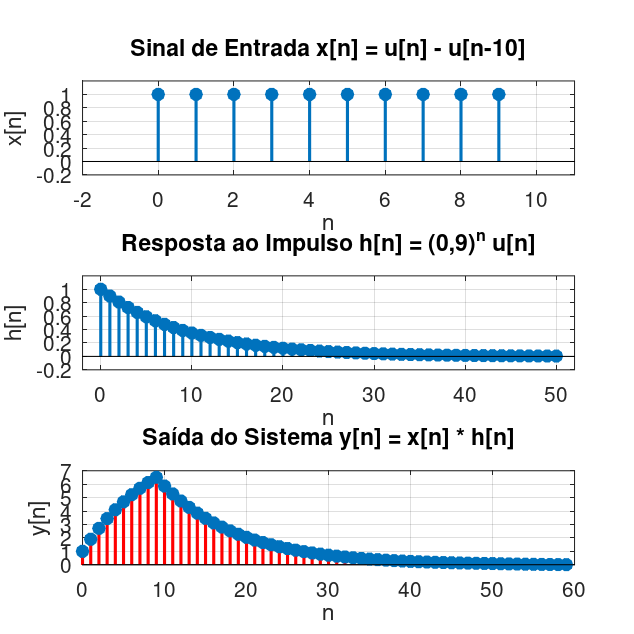
\includegraphics[width=0.9\textwidth]{figuras/parte1.png}
\caption{Entrada, Resposta ao Impulso e Saída do Sistema.}\label{fig:p1}
\end{figure}

\section{Resultados da Parte II: Verificação de Propriedades}
O script desenvolvido calculou a norma da diferença entre os dois lados de cada igualdade das propriedades. Os erros obtidos foram da ordem de $10^{-13}$ a $10^{-15}$, o que comprova numericamente a validade das propriedades (os valores não são zero absoluto devido à precisão de ponto flutuante do computador).

\lstinputlisting[language=Matlab, caption={{Verificação das propriedades.}}]{codigos/parte2.m}

Os resultados numéricos exibidos no terminal foram:
\begin{itemize}
    \item \textbf{Erro Comutação}: $1,7268 \times 10^{-14}$
    \item \textbf{Erro Associação}: $4,1591 \times 10^{-13}$
    \item \textbf{Erro Distribuição}: $5,4578 \times 10^{-14}$
    \item \textbf{Erro Identidade}: $0,0000$
\end{itemize}

Abaixo, a comparação visual da propriedade comutativa:
\begin{figure}[H]
\centering
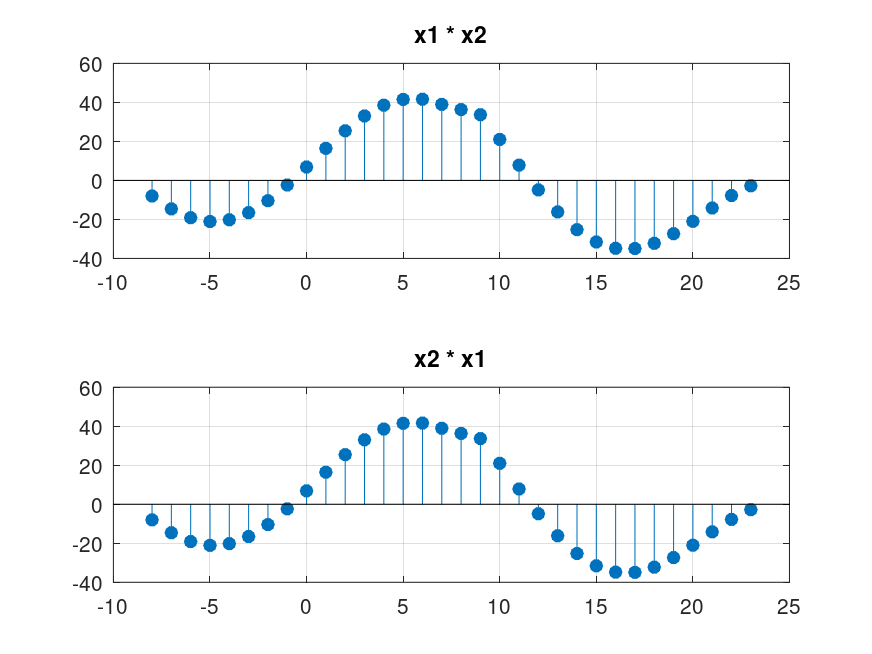
\includegraphics[width=0.8\textwidth]{figuras/parte2_comutacao.png}
\caption{Verificação visual da propriedade Comutativa ($x_1*x_2$ vs $x_2*x_1$).}\label{fig:p2}
\end{figure}

\chapter{Conclusão}

Este laboratório permitiu a consolidação prática dos conceitos de Convolução Linear. Através da implementação da função \texttt{conv\_m}, foi possível compreender como o suporte temporal de sinais discretos é afetado pela operação de convolução, um detalhe crucial que a função padrão \texttt{conv} omite.

As verificações das propriedades de comutação, associação e distribuição reforçaram a estrutura algébrica da convolução, que se comporta de forma análoga à multiplicação de polinômios. A propriedade da identidade (convolução com o impulso unitário deslocado) demonstrou como o sistema identidade apenas translada o sinal no tempo.

O uso do Octave \cite{octaveman} mostrou-se eficiente para o processamento numérico e visualização de sinais, permitindo uma transição suave entre a teoria matemática e a experimentação computacional em Processamento Digital de Sinais.

% ----------------------------------------------------------------------------------------------------- %
\backmatter 
\singlespacing   
% ----------------------------------------------------------------------------------------------------- %
\bibliography{relatorio_3}

\end{document}
